\chapter{Continuo monodimensionale}



Una volta fissata una configurazione $\Omega$ e una deformazione $\fb(\Omega)$,  affrontiamo il problema di modellare le interazioni meccaniche che le accompagnano, sia tra parti di $\Omega$ che tra $\Omega$ e l'ambiente circostante.  


\section{Sistemi di forze}
I tipi più semplici di interazioni meccaniche sono descritti dalle \textit{forze}. Nel tempo sono state sviluppate varie nozioni di  \textit{sistema di forze}, con l'obiettivo di  astrarre dall'esperienza, e quindi riflettere in un modello, un insieme di tratti salienti  sul corpo e sull'ambiente in esame, sia separatamente quando entrino in contatto. 

Il mondo intorno a noi offre esempi di azioni di superficie su un corpo, come l'azione del vento su una vela; e azioni di volume a distanza, come la gravità. La creazione di una nozione di sistema di forze che tenga conto in modo efficiente di tali interazioni superficie-contatto e volume-distanza, così come la creazione della relativa nozione di tensione, è essenzialmente dovuta ad Euler e Cauchy.

Data una configurazione $\Omega$, che identifichiamo con l'intervallo $(x_a, x_b)$, un sistema di forze (di Cauchy) si compone dunque formalmente di due campi:
\begin{itemize}
	\item le forze a \textit{distanza} $\bb(x)=b(x)\eb$ , che agiscono in $\Omega$;
	\item le forze di \textit{contatto} $\sb(x)=s(x)\eb$, che agiscono sulla frontiera di $\Omega$, e dunque nei punti $\{x_a\}$ e $\{x_b\}$.
\end{itemize}

Definiamo \textit{risultante} delle forze che agiscono in $\Omega$ come
\begin{definition}
	\begin{equation}
\rb(\Omega)=r(\Omega)\eb=\int_{\Omega}\bb(x) \dd x+\sb(x_a)+\sb(x_b).
\end{equation}
\end{definition}
Osserviamo che il campo $\bb$ rappresenta una forza per unità di lunghezza.

%Diciamo che il sistema di forze che agiscono in $\bar{\Omega}$ è \textit{bilanciato} se e solo se
%\begin{equation}
%\rb(\Omega)=\mathbf{0}.
%\end{equation}



\section{Le azioni interne}
Cruciale nella descrizione dei corpi continui \textit{à la} Cauchy è la nozione di azione interna (o interazione di contatto). L'idea, che risale ad Eulero, è quella di considerare, all'interno dell'insieme $\Omega$ una sua parte e rendersi conto questa scambia con la parte complementare delle interazioni, che vanno caratterizzate. Questa caratterizzazione qualifica in maniera specifica la classe di corpi continui che consideriamo. In questa trattazione ci occuperemo solo dei cosiddetti \textit{continui di Cauchy}, che però non estinguono la classe di modelli esistenti per caratterizzare le interazioni di contatto.

\begin{figure}[h]
	\centering
	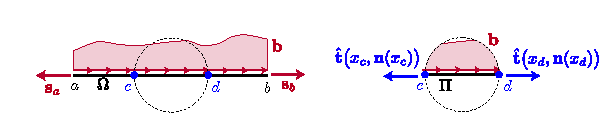
\includegraphics[scale=1.3]{figure/equilibrio/eulero1d}
	\caption{Tagli di Eulero}
	\label{fig:eulero1d}
\end{figure}


Definiamo dunque un sottoinsieme $\Pi\subset\Omega$, che identifichiamo con l'intervallo aperto$(x_c, x_d)$, che individua dunque una \textit{parte} di $\Omega$. In corrispondenza dei punti $x_c$ e $x_d$, la parte $\Pi$ scambia con la parte complementare $\Omega \setminus \Pi$ una forza, che è un'azione di contatto e che denominiamo \textit{azione interna} $\tb$; l'assunzione che nei modelli di Cauchy è che questa azione dipenda non soltanto dal punto, ma anche dalla normale esterna $\nb(x)$ all'insieme, ovvero $\tb=\hat\tb\big(x,\nb(x)\big)$. Nel modello elementare monodimensionale che stiamo considerando $\nb(x_d)=\eb$, mentre $\nb(x_c)=-\eb$.

Possiamo quindi definire il risultante delle forze che agiscono in $\bar{\Pi}$ come 
\begin{equation}
	\rb(\Pi)=r(\Pi)\eb=\int_{\Pi}\bb(x) \dd x+\hat\tb\big(x_c, \nb(x_c)\big)+\hat\tb\big(x_d, \nb(x_d)\big).
\end{equation}
e introdurre l'\textit{assioma di Eulero}: un sistema di forze è bilanciato se e soltanto se
\begin{equation}\label{Euax1}
\rb(\Pi)=\mathbf{0} \qquad \forall \Pi\subset\Omega.
\end{equation}
La richiesta che il risultante sia nullo per ogni parte è naturalmente più forte della sola richiesta che valga per tutto $\Omega$.

Caratterizziamo meglio l'interazione di contatto $\tb$. Per farlo, consideriamo un intervallo centrato in $x$ di ampiezza $2\varepsilon$. Per l'assioma di Eulero, dev'essere:
\begin{equation}
\int_{x-\varepsilon}^{x+\varepsilon}\bb(y)\dd y+\hat{\tb}(x+\varepsilon,\eb)+\hat{\tb}(x-\varepsilon,-\eb)= \mathbf{0}.
\end{equation}
Il primo addendo è dell'ordine $O(\varepsilon)$; facendo dunque tendere a 0 la dimensione dell'intervallo, si ottiene
\begin{definition}
	\begin{equation}\label{lemmaC1}
	\hat{\tb}(x,\eb)=-\hat{\tb}(x,-\eb),
\end{equation}
\end{definition}
un risultato noto come \textit{lemma di Cauchy},  e che traduce nel nostro contesto il principio di \textit{azione e reazione}. L'interazione di contatto è dunque una funzione dispari della normale esterna al dominio.

Un risultato fondamentale nella meccanica dei continui è che l'interazione di contatto è lineare in $\nb$; nel caso tridimensionale, questo è il cosiddetto \textit{teorema di Cauchy}. Dimostriamolo in questo caso elementare monodimensionale. Poiché la mappa $\tb=\hat{\tb}(\cdot, \nb)$ è definita sullo spazio dei vettori unitari, per mostrarne la linearità, è necessario estenderla, assumendo che sia continua,  a tutto lo spazio dei vettori come segue:
\begin{equation}\label{ttext}
	\tb(\vb)=
	\begin{cases}|\vb|\tb\left(\dfrac{\vb}{|\vb|}\right)&\mathrm{~se~}\vb\neq\mathbf{0},\\[.2cm]
		0&\mathrm{~se~}\vb=\mathbf{0},
	\end{cases}
\end{equation}
con $\vb$ non necessariamente unitario. Occorre mostrare allora che valgono le seguenti relazioni:
\begin{enumerate}[label=(R\arabic*)]
	\item $\tb(\alpha \vb)=\alpha\tb(\vb) \quad \forall \alpha, \vb$
	\item $\tb(\vb_1+\vb_2)=\tb(\vb_1)+\tb(\vb_2) \quad \forall \vb_1,\vb_2$.
\end{enumerate}
Osserviamo che se $\alpha=0$ o $\vb =\mathbf{0}$, o se $\alpha>0$ e $\vb \neq \mathbf{0}$, allora (R1) segue direttamente dalla definizione \eqref{ttext}. Consideriamo allora il caso $\alpha<0$ e $\vb_1\neq\mathbf{0}$. Poiché $\alpha=-|\alpha|$,
\begin{equation}
\tb(\alpha \vb)=|\alpha||\vb|\tb\left( \frac{\alpha}{|\alpha|}\frac{\vb}{|\vb|} \right)=|\alpha||\vb|\tb\left(-\frac{\vb}{|\vb|} \right);
\end{equation}
facendo appello al lemma di Cauchy \eqref{lemmaC1}
\begin{equation}
	\tb(\alpha \vb)=|\alpha||\vb|\tb\left(-\frac{\vb}{|\vb|} \right)=-|\alpha||\vb|\tb\left(\frac{\vb}{|\vb|} \right)=\alpha|\vb|\tb\left(\frac{\vb}{|\vb|} \right)=\alpha \tb(\vb),
\end{equation}
e dunque resta dimostrata la (R1). Inoltre, poiché in 1D tutti i vettori sono linearmente dipendenti, allora la dimostrazione di (R2) si riduce a quella di (R1). Non sarà così nel caso 3D, in cui infatti la dimostrazione è molto più delicata. Osserviamo infine che la linearità è diretta conseguenza dell'applicazione del lemma di Cauchy, che è di fatto una relazione di bilancio. 


Resta dunque dimostrato che il vettore delle azioni interne $\tb=\hat{\tb}(x,\nb(x))$ è lineare in $\nb$, ovvero esiste un tensore del secondo ordine $\Tb$, detto \textit{tensore degli sforzi di Cauchy} tale che
\begin{definition}
	\begin{equation}
\hat{\tb}(x,\nb(x))=\Tb(x)\nb(x), \qquad \Tb(x)=T(x) \eb \otimes \eb.
\end{equation}
\end{definition}
Il vettore $\hat{\tb}(x,\nb(x))$ e il tensore $\Tb(x)$ forniscono dunque le stesse informazioni meccaniche.


\begin{remark}
	Si potrebbe pensare che l'estensione di $\tb$ a tutti i vettori di $\Vc$ sia, in luogo di \eqref{ttext}, la seguente:
	\begin{equation}
		\tb(\vb)=
		\begin{cases}\tb\left(\dfrac{\vb}{|\vb|}\right)&\mathrm{~if~}\vb\neq\mathbf{0},\\[.2cm]
			0&\mathrm{~if~}\vb=\mathbf{0}.
		\end{cases}
	\end{equation}
Tuttavia, questa definizione non garantisce la continuità di $\tb(\vb)$ in $\vb=\mathbf{0}$.  Infatti, per garantirne la continuità, dovrebbe essere
\begin{equation}
\lim_{\vb\to\mathbf{0}}\tb(\vb)=\tb(\mathbf{0})=\mathbf{0}.
\end{equation}
Tuttavia, per $\vb\neq \mathbf{0}$,  $\tb\left(\dfrac{\vb}{|\vb|}\right)$ potrebbe non tendere a $\mathbf{0}$, pur ammettendo che sia limitato. Per garantire la continuità in generale, è dunque necessario  che l'estensione abbia la forma data da \eqref{ttext}.
\end{remark}


\section{Equazione puntuale di equilibrio}
L'assioma di Eulero \eqref{Euax1} fornisce un'informazione di equilibrio globale per la parte $\Pi$.  vogliamo adesso determinare delle informazioni che siano invece di natura puntuale, come avviene in tutte le teorie di campo. Per farlo utilizzeremo la solita tecnica: sceglieremo un parte infinitesima attorno ad un punto, richiederemo che l'assioma di Eulero sia soddisfatto e faremo tendere a zero la dimensione della parte. In 1D questa operazione è particolarmente semplice; qualche accortezza in più dovremo utilizzare nel capitolo successivo, quando ci occuperemo del modello tridimensionale.

\tR{da rivedere}
Più precisamente,  utilizzeremo il seguente \textit{lemma di localizzazione}: se $\Ic_\varepsilon\coloneqq[x_0, x_0+\varepsilon] \}$  e $g$ una funzione continua in un intorno di $x_0$, allora
\begin{equation}\label{loc1}
	\lim_{\varepsilon\to 0}\frac{1}{\varepsilon}\int_{\Ic_\varepsilon}g(x)\dd x=g(x_0).
\end{equation}

\begin{remark}

	Per dimostrare vero il lemma di localizzazione, consideriamo l'integrale
	\[
	\frac{1}{\varepsilon} \int_{x_0}^{x_0 + \varepsilon} g(x) \, \dd x.
	\]
	
	Per qualsiasi \(\delta > 0\), poiché \(g\) è continua in \(x_0\), esiste un \(\eta > 0\) tale che \( |g(x) - g(x_0)| < \delta \) per tutti \(x\) in \([x_0, x_0 + \eta]\).
	%
	Scegliamo \(\varepsilon\) sufficientemente piccolo, quindi \(\varepsilon < \eta\). Allora, per \(x \in [x_0, x_0 + \varepsilon]\), abbiamo che \( |g(x) - g(x_0)| < \delta \).
	Pertanto possiamo scrivere:
	%
	\[
	\left| \frac{1}{\varepsilon} \int_{x_0}^{x_0 + \varepsilon} (g(x) - g(x_0)) \, \dd x \right| \leq \frac{1}{\varepsilon} \int_{x_0}^{x_0 + \varepsilon} |g(x) - g(x_0)| \, \dd x < \frac{1}{\varepsilon} \int_{x_0}^{x_0 + \varepsilon} \delta \, \dd x=\delta.
	\]
%
Poiché \(\delta\) è arbitrariamente piccolo, possiamo concludere che
		\[
	\lim_{\varepsilon \to 0} \frac{1}{\varepsilon} \int_{x_0}^{x_0 + \varepsilon} g(x) \, \dd x = g(x_0).
	\]
\end{remark}

\subsection{Relazione di Cauchy per punti interni}
Iniziamo considerando un punto $x$ interno al segmento $\Omega=(x_a, x_b)$ che rappresenta una configurazione del corpo e definiamo un intervallo $\Ic_\varepsilon\coloneqq [x,x+\varepsilon]$ , in modo che $\Ic_\varepsilon\subset\Omega$. L'assioma di Eulero diventa dunque
\begin{equation}
\mathbf{0}=\rb(\Ic_\varepsilon)=\int_{\Ic_\varepsilon}\bb(y)\dd y+\hat\tb(x+\varepsilon,\eb)+\hat{\tb}(x,-\eb),
=\int_{\Ic_\varepsilon}\bb(y)\dd y+\hat\tb(x+\varepsilon,\eb)-\hat{\tb}(x,\eb),
\end{equation}
dove si è fatto uso del lemma di Cauchy. Facendo appello alla rappresentazione data dal teorema di Cauchy, dividendo per la misura dell'intervallo $\Ic_\varepsilon$, si ha
\begin{equation}
\left( \frac{1}{\varepsilon}\int_{\Ic_\varepsilon}b(y)\dd y+\frac{T(x+\varepsilon)-T(x)}{\varepsilon}\right)\,\eb=\mathbf{0};
\end{equation}
facendo tendere adesso $\varepsilon$ a 0 e appellandosi al lemma di localizzazione \eqref{loc1}, si ottiene
\begin{definition}
	\begin{equation}\label{EPQ1}
	\big(b(x)+T'(x)\big)\eb=\mathbf{0},
\end{equation}
\end{definition}
 che rappresenta, nel caso 1D, l'\textit{equazione puntuale di equilibrio}, o relazione di Cauchy per punti interni.  La \eqref{EPQ1} può essere riscritta in termini del tensore degli sforzi di Cauchy come
\begin{definition}
	\begin{equation}
\bb(x)+\Div\Tb(x)=\mathbf{0},
\end{equation}
\end{definition}
essendo
\begin{equation}
\Div\Tb(x)=\Tb,_x(x)\,\eb=\big(T'(x)  \,\eb\otimes \eb\big)\eb=T'(x)\,  \eb.
\end{equation}

\subsection{Relazione di Cauchy per punti di frontiera}
Consideriamo adesso un punto $x$ che si trova sulla frontiera di $\Omega=(x_a, x_b)$, ad esempio fissiamo $x=x_b$. Definiamo l' intervallo di ampiezza $\varepsilon$ dato da $\Ic_\varepsilon=(x_b-\varepsilon, x_b)$. L'assioma di Eulero assume adesso la seguente forma:
\begin{equation}
\mathbf{0}=\rb(\Ic_\varepsilon)=\int_{\Ic_\varepsilon}\bb(y)\dd y+\hat\tb(x_b-\varepsilon,-\eb)+\sb(x_b).
\end{equation}
Facendo uso del lemma di Cauchy, si ottiene che
\begin{equation}
\int_{\Ic_\varepsilon}\bb(y)\dd y-\hat\tb(x-\varepsilon,\eb)+\sb(x_b).
\end{equation}
Facendo tendere a 0 l'ampiezza $\varepsilon$ dell'intervallo, dato che $\int_{\Ic_\varepsilon}\bb(y)\dd y=O(\varepsilon)$, se ne ricava che
\begin{equation}
\hat\tb(x_b,\eb)=\sb(x_b), \qquad \Longleftrightarrow\quad T(x_b)=s(x_b).
\end{equation}
In maniera del tutto analoga si ricava
\begin{equation}
	\hat\tb(x_a,\eb)=\sb(x_a), \qquad \Longleftrightarrow \quad -T(x_a)=s(x_a).
\end{equation}
Utilizzando la rappresentazione tramite il tensore degli sforzi di Cauchy, queste due relazioni possono essere scritte come
\begin{definition}
	\begin{equation}
\Tb(x)\nb(x)=\sb(x), \quad \textrm{per} \;\; x=x_a \;\;\textrm{o} \;\;  x=x_b.
\end{equation}
\end{definition}
Questa relazione, valida per punti di frontiera, specifica che il valore dell'interazione di contatto che si registra sulla frontiera deve eguagliare le forze di superficie colà applicate.

Riassumendo, assegnati i campi di forze di volume $\bb(x)$ e di superficie $\sb(x)$ le azioni interne, descritte tramite $\hat\tb(x, \nb) $ o, equivalentemente tramite il tensore di Cauchy $\Tb(x)$ devono soddisfare le relazioni:
\begin{equation}
\begin{cases}
	\begin{array}{ll}
		\Div\Tb +\bb= \mathbf{0}, & \qquad \text{in}\;\; \Omega \\
		\Tb\nb=\sb, & \qquad \text{in}\;\; \partial\Omega,
	\end{array}
\end{cases}
\end{equation}
che costituiscono il \textit{problema statico}, equivalente, nel presente contesto 1D, a
\begin{equation}
	\begin{cases}
		\begin{array}{ll}
		T'(x)+b(x)=0, \quad  x\in(x_a,x_b) \\
		-T(x_a)=s(x_a),\;\;T(x_b)=s(x_b).
		\end{array}
	\end{cases}
\end{equation}



\section{Lavoro di un sistema di forze}\label{ELV1D}
Nella meccanica ci sono due modi diversi per fornire una rappresentazione matematica del concetto di forza: il primo consiste nel rappresentarla tramite un \textit{vettore} applicato, un ente matematico avente  un'origine, un modulo, una direzione e un verso. L'estensione naturale ai mezzi continui porta alla definizione di campi vettoriali associati a misure, da cui le `forze di volume', `di superficie', `per unità di massa', etc.

Il secondo modo, che risale almeno a d'Alembert, è quello cui normalmente ci si riferisce come metodo dei lavori virtuali. Questo secondo modo è in realtà più naturale del primo, essendo una traduzione in termini matematici di ciò che comunemente si fa nell'esperienza per valutare una forza. Ad esempio, se si desidera conoscere la forza peso di un oggetto, l'operazione più naturale che si fa è `soppesarlo', ovvero imprimere uno spostamento (o una velocità) e valutare quanta `fatica' si fa nell'operazione: il nostro cervello non è in grado di valutare una forza, ma solo il lavoro che essa compie. Da un punto di vista matematico questa procedura si può descrivere così: ad un certo istante, si considera sul sistema $\Pc$ un campo vettoriale $\ub$ che definisce, a quell'istante, uno \textit{spostamento virtuale}; le forze che producono questo spostamento sono note se è noto il loro `lavoro virtuale'. 
%Ancora più precisamente  --- e astrattamente  ---  si considera un insieme $\Uc$ di spostamenti virtuali $\delta\ub$, dove $\Uc$ è uno spazio dotato di norma, e si afferma di conoscere le forze esercitate su un sistema se esiste un funzionale lineare $\Lc(\Pc)[\delta\ub]$, il cui valore, per ogni $\delta\ub$, è uguale al lavoro virtuale prodotto dalle forze durante il moto definito da $\delta\ub$.

%L'idea fondamentale che sta alla base di questo secondo modo di vedere le cose è quella di \textit{dualità}. Uno dei vantaggi di questo secondo modo di procedere risiede senz'altro nella possibilità di definire in maniera piuttosto libera lo spazio $\Uc$, in modo da avere una descrizione più o meno fine del moto del sistema: è quel che abbiamo fatto all'inizio dello studio della cinematica della trave, in cui lo spazio degli spostamenti virtuali è quello indotto dalla cinematica dei corpi a forma di trave, che richiedeva una descrizione dello spostamento dei punti della linea d'asse e della rotazione locale della sezione trasversale. Una volta fissato $\Uc$, l'insieme delle forze definisce a sua volta lo spazio vettoriale $\Uc^\star$, il \textit{duale} di $\Uc$.

%Occorre ammettere che la nozione di funzionale lineare definito su uno spazio vettoriale è  più astratta e complessa di quella di un campo vettoriale, motivo per cui la prima descrizione della nozione di forza è quella che, almeno all'inizio, è prevalsa. Inoltre, nel momento in cui è apparsa questa idea, la nozione di dualità, che può essere vista come un precursore della nozione di \textit{misura} e di \textit{distribuzione}, non era ancora stata sviluppata appieno. Oggigiorno l'analisi funzionale e le sue applicazioni alla meccanica hanno fornito strumenti matematici notevoli alla nozione di dualità sicché, a partire almeno dalla metà del secolo scorso, l'utilizzo degli strumenti connessi all'idea di lavoro virtuale e dualità è stata estremamente feconda nello sviluppo delle teorie di campo.

%In questo capitolo intendiamo mettere in luce gli aspetti meccanici che la nozione di dualità indotta da quella del lavoro virtuale  porta con sé, nel caso dei corpi continui a forma di trave.

Di seguito utilizzeremo il concetto di \textit{lavoro virtuale}, che nel contesto della meccanica puntiforme può essere definito come segue: se $\pb$ è una forza che agisce su un punto e $\ub$ è un qualunque spostamento del punto (non necessariamente quello prodotto dalla forza $\pb$), allora la quantità $\pb \cdot \ub$ rappresenta il lavoro virtuale che la forza $\pb$ compie sullo spostamento $\ub$. In sostanza, il termine virtuale indica che non esiste necessariamente una ``corrispondenza'' tra forza e spostamento.

Sia  $\Omega\supset\Pi=(x_a, x_b)$ soggetto ad un sistema di forze $(\bb, \sb)$; su $\Pi$ assumiamo che sia definito un campo di spostamento $\ub$. Si definisce lavoro esterno, compiuto dal sistema di forze sullo spostamento dato, 
\begin{definition}
	\begin{equation}\label{Le1}
\Lc_e(\Omega)\coloneqq\int_{\Omega}\bb(x)\cdot \ub(x)\dd x+\sb(x_a)\cdot\ub(x_a)+\sb(x_b)\cdot\ub(x_b),
\end{equation}
\end{definition}
che generalizza, nel presente contesto 1D, il lavoro di un punto materiale.


\section{Equazione dei lavori virtuali}
Consideriamo una coppia $\{\Eb, \ub\}$ di deformazione e spostamento. Diciamo che $\{\Eb, \ub\}$  è compatibile, o congruente, se
\begin{equation}
	\Eb =\sym \nabla \ub,
\end{equation}
ovvero
\begin{equation}\label{cong1}
	E(x)=u'(x).
\end{equation}

Naturalmente è sempre possibile trovare $\Eb$, tale che $\{\Eb, \ub\}$  sia compatibile; il contrario non è sempre vero, perché non è detto che, data $\Eb$ esista un campo $\ub$ tale che $\Eb =\sym \nabla \ub$.

Consideriamo adesso la terna $\{\Tb, \bb, \sb\}$ di sforzo, forze di volume e di contatto; diciamo che la terna  è equilibrata se
\begin{equation}
\begin{cases}
	\begin{array}{ll}
		\Div\Tb +\bb= \mathbf{0}, & \qquad \text{in}\;\; \Omega \\
		\Tb\nb=\sb, & \qquad \text{in}\;\; \partial\Omega,
	\end{array}
\end{cases}
\end{equation}
ovvero
	\begin{equation}\label{bil1}
		\begin{cases}
			\begin{array}{ll}
				T'(x)+b(x)=0, \quad  x\in(x_a,x_b) \\
				-T(x_a)=s(x_a),\;\;T(x_b)=s(x_b).
			\end{array}
		\end{cases}
\end{equation}

Vale il seguente 
\begin{definition}
\textbf{\textit{Teorema dei Lavori Virtuali}}. Sia $\{\Eb, \ub\}$  una coppia congruente e sia $\{\Tb, \bb, \sb\}$ una terna equilibrata. Allora il \textit{lavoro virtuale esterno}
\begin{equation}
\begin{aligned}
	\Lc_e(\Omega)&\coloneqq\int_{\Omega}\bb(x)\cdot \ub(x)\dd x+\sb(x_a)\cdot\ub(x_a)+\sb(x_b)\cdot\ub(x_b)\\
	&=\int_{x_a}^{x_b}b(x)u(x)\dd x+s(x_a)u(x_a)+s(x_b)u(x_b)
\end{aligned}
\end{equation}
è uguale al lavoro \textit{virtuale interno }
	\begin{equation}
\Lc_i(\Omega)=\int_{\Omega}\Tb(x)\cdot \Eb(x)=\int_{x_a}^{x_b}T(x) E(x)\dd x
\end{equation}
\end{definition}

È cruciale osservare che, in generale, non c'è  alcun legame tra la coppia $\{\Eb, \ub\}$ e la terna $\{\Tb, \bb, \sb\}$, motivo per cui il lavoro è detto `virtuale'.

Per dimostrarlo, partiamo dall'espressione del lavoro esterno che, utilizzando la \eqref{bil1}$_2$ e il teorema fondamentale del calcolo integrale, può essere così scritto:
\begin{equation}
\begin{aligned}
\Lc_e(\Omega)&=\int_{x_a}^{x_b}b(x)u(x)\dd x-T(x_a)u(x_a)+T(x_b)u(x_b)\\
&=\int_{x_a}^{x_b}\big( b(x)u(x)+ \big(T(x)u(x)\big)' \,\big)\dd x\\
&=\int_{x_a}^{x_b}\big(\big(b(x)+T'(x)\big) u(x)+T(x)u'(x)\big) \dd x.
\end{aligned}
\end{equation}
Invocando adesso l'equazione di bilancio \eqref{bil1}$_1$, notiamo che il primo addendo dell'integranda è nullo; usando l'equazione di congruenza  \eqref{cong1}, concludiamo allora che 
\begin{equation}
\begin{aligned}
	\Lc_e(\Omega)=\int_{x_a}^{x_b}T(x) E(x)\dd x=	\Lc_i(\Omega).
\end{aligned}
\end{equation}

Abbiamo dunque dimostrato quello che abbiamo definito \textit{Teorema dei Lavori Virtuali}, ovvero, in maniera schematica
\begin{definition}
	\begin{equation}
	\left.\begin{array}{rr}\{\mathbf{E},\mathbf{u}\}\text{ congruente }\\\{\mathbf{T},\mathbf{b},\mathbf{s}\}\text{ equilibrata }\end{array}\right\}\quad\Longrightarrow\quad\mathcal{L}_i=\mathcal{L}_e.
\end{equation}
\end{definition}

L'equazione dei lavori virtuali può assurgere a principio, nel senso che, piuttosto che postulare che siano validi gli assiomi di Eulero, è possibile caratterizzare un sistema bilanciato direttamente in termini di lavoro. Infatti vale il seguente teorema, scritto in maniera schematica come 
\begin{definition}
	\begin{equation}
	\mathcal{L}_i=\mathcal{L}_e\quad\forall\{\mathbf{E},\mathbf{u}\}\text{ congruente}\quad\Longrightarrow\quad\{\mathbf{T},\mathbf{b},\mathbf{s}\}\text{ equilibrata.}
\end{equation}
\end{definition}
In altri termini, la pretesa che il lavoro virtuale interno sia uguale al lavoro virtuale esterno, per ogni coppia $\{\mathbf{E},\mathbf{u}\}$ congruente,  implica l'equilibrio, ovvero la terna $\{\mathbf{T},\mathbf{b},\mathbf{s}\}$ è equilibrata.

Per dimostrarlo, partiamo ovviamente dal richiedere che 
\begin{equation}\label{elc1}
\int_{x_a}^{x_b}T(x) E(x)\dd x=\int_{x_a}^{x_b}b(x)u(x)\dd x+s(x_a)u(x_a)+s(x_b)u(x_b).
\end{equation}
Utilizzando l'equazione di congruenza e il teorema fondamentale del calcolo integrale,  il lavoro interno può essere scritto come segue:
\begin{equation}
	\begin{aligned}
	\int_{x_a}^{x_b}T(x) E(x)\dd x&=\int_{x_a}^{x_b}T(x) u'(x)\dd x=	\int_{x_a}^{x_b}\big( T(x)u(x)   \big)'-T'(x)u(x)\big)\dd x\\
	&=T(x_b)u(x_b)-T(x_a)u(x_a)-\int_{x_a}^{x_b}T'(x)u(x)\dd x.
	\end{aligned}
\end{equation}
La \eqref{elc1} allora implica che
\begin{equation}
\big( T(x_b)-s(x_b) \big)u(x_b)+\big( -T(x_a)-s(x_a) \big)u(x_a)+\int_{x_a}^{x_b}\big(  -T'(x) -b(x)\big)u(x) \dd x=0,
\end{equation}
che dev'essere valida per ogni campo di spostamento $u(x)$ e dunque
\begin{equation}
T(x_b)=s(x_b), \quad -T(x_a)=s(x_a), \quad T'(x) +b(x)=0,
\end{equation}
ovvero la terna $\{\Tb, \bb, \sb\}$ è equilibrata.

Possiamo infine far vedere che vale anche la terza delle combinazioni possibili:
\begin{definition}
	\begin{equation}
	\mathcal{L}_i=\mathcal{L}_e\quad\forall\{\mathbf{T},\mathbf{b},\mathbf{s}\}\text{ equilibrata}\quad\Longrightarrow\quad\{\mathbf{E},\mathbf{u}\}\text{ congruente.}
\end{equation}
\end{definition}
Infatti, poiché la terna è equilibrata valgono le \eqref{bil1} e dunque
\begin{equation}
	\begin{aligned}
\int_{x_a}^{x_b}T(x)E(x)\dd x&=\int_{x_a}^{x_b}b(x)u(x)\dd x+s(x_a)u(x_a)+s(x_b)u(x_b)\\
&=\int_{x_a}^{x_b}-T'(x)u(x)\dd x-T(x_a)u(x_a)+T(x_b)u(x_b)\\
&=\int_{x_a}^{x_b}\big(-\big( T(x)u(x) \big)'+T(x)u'(x)\dd x-T(x_a)u(x_a)+T(x_b)u(x_b)\\
&=\int_{x_a}^{x_b}T(x)u'(x)\dd x.
\end{aligned}
\end{equation}
Pertanto risulta che
\begin{equation}
\int_{x_a}^{x_b}T(x)\big(E(x)-u'(x)\big)\dd x,
\end{equation}
valida per ogni $T(x)$, il che è sufficiente a concludere che $E(x)=u'(x)$, e dunque la coppia $\{\Eb, \ub\}$ è congruente.


Equilibrio, Congruenza e Lavori Virtuali rappresentano dunque una sorta di `trinità' meccanica tale che, dati due elementi, il terzo ne è conseguenza. 

	\begin{center}

	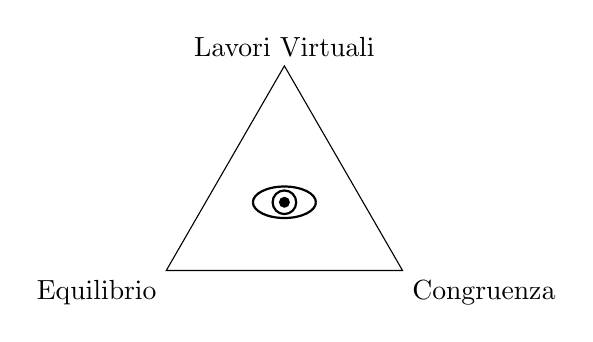
\begin{tikzpicture}
		% Coordinates of the triangle vertices
		\coordinate (A) at (0,0);
		\coordinate (B) at (3,0);
		\coordinate (C) at (1.5,2.598); % 2.598 is approximately 3*sin(60 degrees)
		
		% Draw the triangle
		\draw (A) -- (B) -- (C) -- cycle;
		
		% Labels
		\node[below left] at (A) {Equilibrio};
		\node[below right] at (B) {Congruenza};
		\node[above] at (C) {Lavori Virtuali};
		
		% Calculate the centroid of the triangle
		\coordinate (Centroid) at (1.5,0.866); % Centroid of an equilateral triangle
		
		% Draw an almond-shaped eye at the centroid
		\draw[thick] (Centroid) ++(-0.4, 0) arc[start angle=180, end angle=360, x radius=0.4, y radius=0.2];
		\draw[thick] (Centroid) ++(0.4, 0) arc[start angle=0, end angle=180, x radius=0.4, y radius=0.2];
		
		% Draw the iris
		\draw[thick] (Centroid) circle (0.15);
		
		% Draw the pupil
		\fill (Centroid) circle (0.07);
		
	\end{tikzpicture}
		\end{center}

